\documentclass[a4paper,10pt]{article}
\usepackage[english]{babel}
\usepackage[utf8]{inputenc}
\usepackage{url}
\usepackage[margin=1in]{geometry}
\usepackage{enumitem}

\setlist[itemize]{leftmargin=1.2in}


\usepackage[nottoc]{tocbibind}
\usepackage{fancyvrb} 
\usepackage{float}
\usepackage{graphicx}
\usepackage{subcaption}
\usepackage{color}
\usepackage{booktabs}
\usepackage{listings}

\title{Combinatorial Optimization\\Homework 2 – Heuristics and Exact Solutions}
\author{Matyáš Skalický\\skalimat@fit.cvut.cz}

\begin{document}
\date{November 11, 2021}
\maketitle
\tableofcontents
\medskip


\section{Implementation}
This report describes implemented dynamic-programming approaches as-well as simple heuristics and FPTAS algorithm. The branch\&bound method implemented in the last exercise was reused for this task.

Implemented algorithms were evaluated on all instances from all datasets up to the instance size of $27$. CPU runtime for each of these tasks was measured.

\subsection{Exact Methods}

The \textbf{branch\&bound} algorithm uses brute-force with 2 speedups. We stop when the current candidate already exceeds the capacity of a bag. Also, we don't recurse further when the cost sum of the items that can be added into the bag is lower than the best found solution.

At first, I've implemented the dynamic programming solution based on the \textbf{decomposition by cost}. This solution was based on memoization by the recursive function calls by returning the maximum value from the tested branches on return.

Only after that I found out that the FPTAS algorithm requires \textbf{decomposition by weight}. I have implemented the dynamic solution based on weight. But this time by iteratively calculating contents of the table. The code was way more complex compared to the original decomposition by cost. At least in terms of readability.

\subsection{Heuristics}

Compared to the exact methods mentioned earlier, heuristics calculate the result faster, but at the cost of the solution being not exact. I will refer to the difference between ideal and resulting cost of the predicted bag as the \emph{error}.

The \textbf{greedy} algorithm simply adds the items with the highest cost/weight ratio until the capacity of the bag is reached. The \textbf{redux} algorithm extends this by also trying to construct the bag with the most valuable item that fits into the bag.

\textbf{FPTAS} algorithm is based on the dynamic decomposition by weight. For a given $\epsilon$ a constant $k$ is computed for each bag. 

\begin{equation}
k = \frac{\epsilon}{|\textrm{items}|} \cdot \Bigg[\max_{i \in \small{\textrm{items}}} i.\textrm{cost}\Bigg]
\end{equation}

Costs of all items in the bag are divided by $k$ and rounded to integral values. This leads to smaller memoization table (and thus faster solution) while keeping the size of the error proportionally small.

\section{Experiments}

\subsection{Exact Algorithms}

\begin{figure}[!htb]
	\centering
  	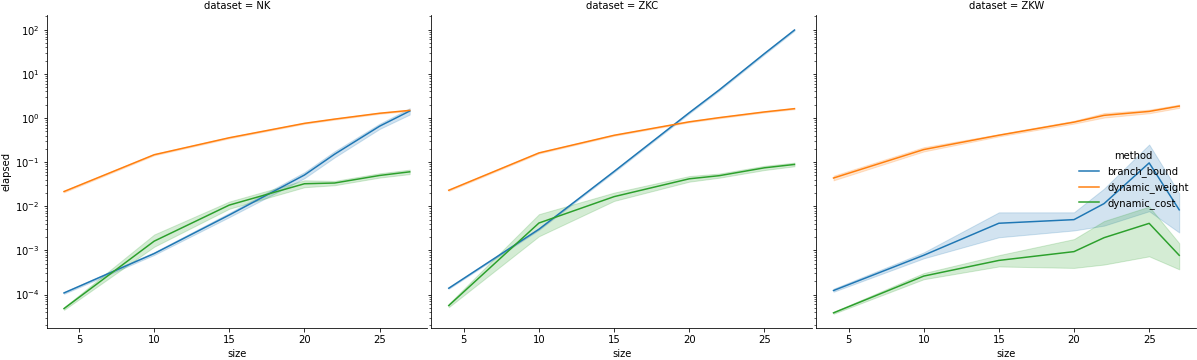
\includegraphics[width=\textwidth]{images/exacts_comparison.png}
	\caption{Comparison of the exact algorithms: branch\&bound, decomposition by cost and weight}
	\label{exacts_comparison}
\end{figure}

As seen from the Figure \ref{exacts_comparison} the branch\&bound algorithm is exponential regarding the instance size. Interestingly enough, for smaller instances, this solution beats the dynamic programming as it doesn't require any expensive setup due to allocation of a memoization table.

Figure \ref{exacts_comparison} also compares dynamic programming using decomposition by cost and decomposition by weight. Decomposition by cost was way faster as it was calculated using a simple implementation without having to initialize the lookup table prior to evaluation. Also, the size of the potential lookup table for weight decomposition is $\textrm{total-item-count} \cdot \textrm{total-items-cost}$ while for cost decomposition it is $\textrm{total-item-count} \cdot \textrm{bag-capacity}$ which can lead to different execution times.

\begin{table}[!htb]
\centering
\begin{tabular}{llrrr}
\toprule
method & dataset &       min &      mean &        max \\
\midrule
branch\&bound & NK &  0.000409 &  0.938218 &  11.052758 \\
dynamic cost & NK &  0.000033 &  0.073039 &   1.012237 \\
dynamic weight & NK &  0.765613 &  1.652262 &   2.376139 \\
greedy simple & NK &  0.000024 &  0.000058 &   0.000287 \\
greedy redux & NK &  0.000034 &  0.000076 &   0.000386 \\
\bottomrule
\end{tabular}
\caption{Runtime for instance size 25 on NK dataset}
\label{exacts_table}
\end{table}

The main reason for speedup of decomposition by cost was the usage of builtin cache from python's \emph{itertools}. Thanks to this, there was no slow initialization.

Overall, both dynamic algorithms seemed to be scaling in a similar way.  Decomposition by weight has just a fixed overhead mentioned earlier. This is further shown in the Table \ref{exacts_table}.

\subsection{Greedy Heuristics}

\begin{figure}[!htb]
	\centering
  	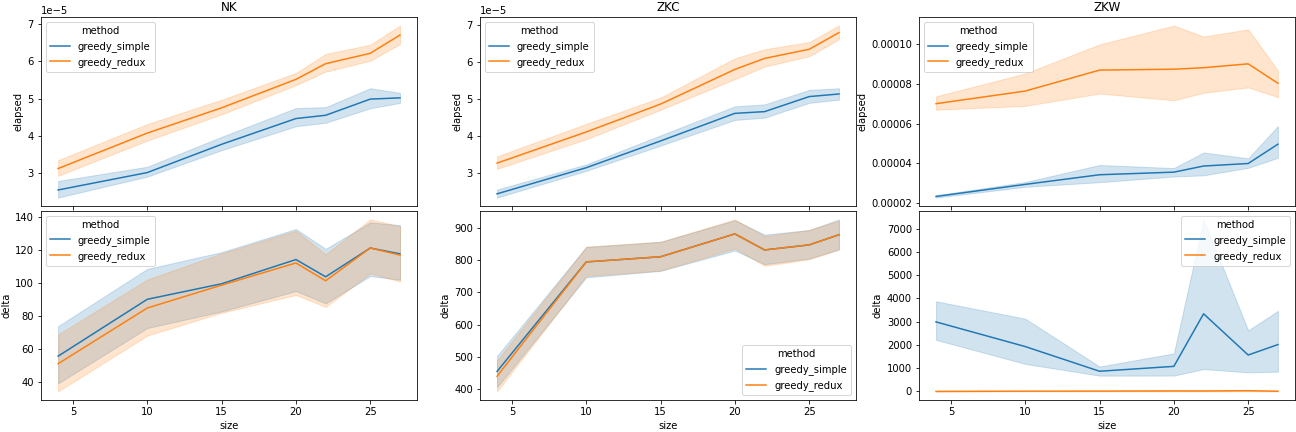
\includegraphics[width=\textwidth]{images/greedy_comparison_datasets.png}
	\caption{Comparison of the greedy heuristics across datasets}
	\label{greedy_comparison_datasets}
\end{figure}

Figure \ref{greedy_comparison_datasets} compares the simple greedy algorithm against the redux version. As expected, redux is always slower than the baseline greedy version. Performance is the same on both NK and ZKC datasets. Redux implementation beats the simple heuristic on the ZKW dataset as this dataset is engineered this way.

\subsection{FPTAS Algorithm}

%\begin{figure}[!htb]
%	\centering
%  	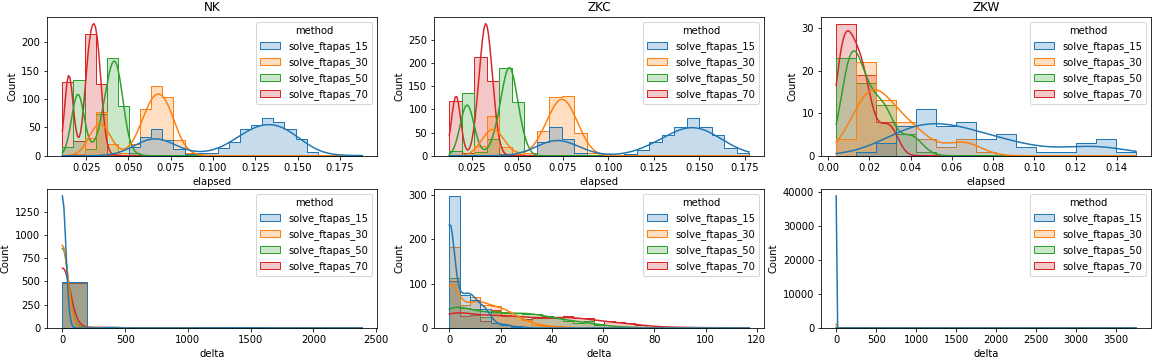
\includegraphics[width=\textwidth]{images/fpatas_datasets.png}
%	\caption{fpatas datasets}
%	\label{Comparison of mean runtime (elapsed) and error size (delta) across datasets}
%\end{figure}

Figure \ref{fptas_comparison} shows the comparison of the FPTAS algorithm across different datasets. As expected, when we change the epsilon value, the mean error decreases, while the mean elapsed time increases. This allows us to precisely set the tradeoff between computation complexity and desired precision.

\begin{figure}[!htb]
	\centering
  	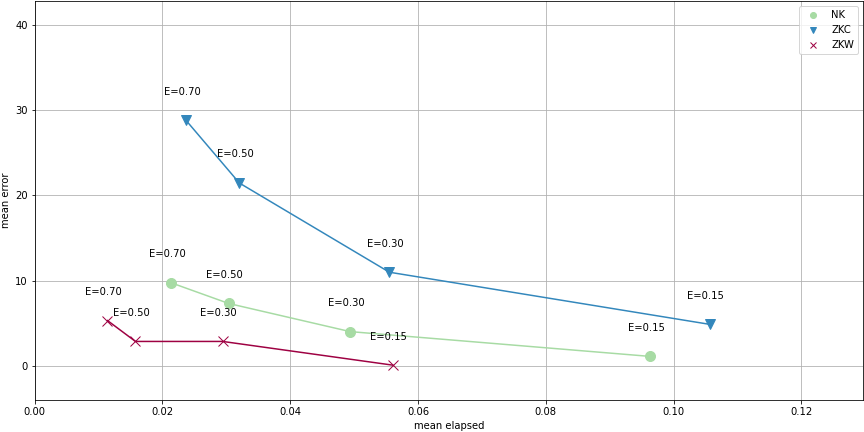
\includegraphics[width=\textwidth]{images/fptas_comparison.png}
	\caption{Comparison of mean runtime (elapsed) and mean error across datasets}
	\label{fptas_comparison}
\end{figure}

Table \ref{fptas_table} describes the relative error and elapsed time for different value of $\epsilon$. Relative error never exceeds the value of $\epsilon$ as expected. 

\begin{table}[!htb]
\centering
\begin{tabular}{llrrrrrr}
\toprule
                &    & \multicolumn{3}{l}{elapsed} & \multicolumn{3}{l}{error} \\
                &    &       min &      mean &       max &   min &      mean &       max \\
method & dataset &           &           &           &       &           &           \\
\midrule
FPTAS 0.15 & NK &  0.000215 &  0.107760 &  0.606508 &   0.0 &  0.000046 &  0.039524 \\
FPTAS 0.30 & NK &  0.000249 &  0.055776 &  0.488715 &   0.0 &  0.000151 &  0.099057 \\
FPTAS 0.50 & NK &  0.000187 &  0.034595 &  0.326600 &   0.0 &  0.000513 &  0.128881 \\
FPTAS 0.70 & NK &  0.000176 &  0.025523 &  0.388467 &   0.0 &  0.000636 &  0.211354 \\
\bottomrule
\end{tabular}
\caption{Basic information about FPTAS algorithm runtime and relative error}
\label{fptas_table}
\end{table}

\section{Discussion and Takeoffs}
Regarding the simple heuristics, the greedy algorithm is extremely fast. On a general dataset, \emph{simple} achieved comparable results to the \emph{redux} algorithm. \emph{Redux} worked better only in for a specific dataset.

It is interesting to note that the dynamic programming solution starts to be viable only from a certain instance size. For smaller instances, it is faster to just utilize a brute-force search with branch\&bound optimizations.

I have implemented the dynamic programming solution using both approaches, by memoizing the recursive calls as well as by iteratively computing the solution. First mentioned method was much simpler to implement and therefore less prone to mistakes.

FPTAS is a nice framework which gives us the power to easily tradeoff desired precision and required computational resources.

I have spent a considerable amount of time debugging an instance where an item cost was $0$ after dividing by $k$ in FPTAS algorithm. This led to a wrong solution even though the exact solutions were correct on all provided data.

Another issue that took me a while to debug was an indexing error when forward-calculating the dynamic solution. A solution where a recursive call is simply cached has its beauty.

\end{document}